%%%%%%%%%%%%%%%%%%%%%%%%%%%%%%%%%%%%%%%%%%%%%%%%%%%%%%%%%%%%
%% Packages
\documentclass[10pt, a4paper]{article}%文件类型article,正文字号10pt
\usepackage[top=3cm, bottom=4cm, left=3.5cm, right=3.5cm]{geometry}%页面布局
\usepackage{amsmath,amsthm,amsfonts,amssymb,amscd, fancyhdr, color, comment, graphicx, environ}
%fancyhdr:页眉页脚
%graphicx:插图
%amsthm:American Mathematical Society (AMS) Style theorem typesetting 定理环境
%amssymb:公式符号 American Mathematical Society (AMS) Style Symbols
%amsmath:数学工具 AMS mathematical facilities
%amscd:communicative diagram
%color:提供对色彩的支持
%comment:插入评论支持
%environ: creating new environments
\usepackage{float}%浮动体
\usepackage{mathrsfs}%RSFS:Ralph Smith's Formal Script font(The fonts provide uppercase ‘formal’ script letters for use as symbols in scientific and mathematical typesetting )
\usepackage[math-style=ISO]{unicode-math}%a complete implementation of unicode maths for XeLaTeX and LuaLaTeX
\usepackage{lastpage}%Reference last page for Page N of M type footers
\usepackage[dvipsnames]{xcolor}%Driver-independent color extensions
\usepackage[framemethod=TikZ]{mdframed}%Framed environments that can split at page boundaries(PStricks or TikZ)
\usepackage{enumerate}%Enumerate with redefinable labels
\usepackage[shortlabels]{enumitem}%Control layout of itemize, enumerate, description
\usepackage{indentfirst}%Indent first paragraph after section header
\usepackage{listings}%Typeset source code
\usepackage{sectsty}%help change the style of any or all of sectional headers
\usepackage{thmtools}% commonly-needed support for typesetting theorems
\usepackage{shadethm}% produce a theorem statement in a shaded box
\usepackage{hyperref}% support for hypertext
\usepackage{setspace}%Set space between lines
\usepackage{lipsum}
\usepackage{appendix}
\usepackage{etoc}
\usepackage{titlesec}
\setmathfont{TeX Gyre Termes Math}
\hypersetup{
    colorlinks=true,
    linkcolor=purple,
    filecolor=magenta,      
    urlcolor=purple,
}


%%%%%%%%%%%%%%%%%%%%%%%%%%%%%%%%%%%%%%%%%%%%%%%%%%%%%%%%%%%%
%% Environment setup
\mdfsetup{skipabove=\topskip,skipbelow=\topskip}%控制mdframed的区域和其他部分的间距
\mdfdefinestyle{theoremstyle}{%define theorem style
linecolor=black,
linewidth=1pt,%
frametitlerule=true,%
frametitlebackgroundcolor=gray!20,
innertopmargin=\topskip,
}
\mdtheorem[style=theoremstyle]{Problem}{Problem}

\definecolor{codegreen}{rgb}{0,0.6,0}
\definecolor{codegray}{rgb}{0.5,0.5,0.5}
\definecolor{codepurple}{RGB}{96,0,89}
\definecolor{backcolour}{rgb}{0.95,0.95,0.92}

\lstdefinestyle{mystyle}{
    backgroundcolor=\color{backcolour},   
    commentstyle=\color{codepurple},
    keywordstyle=\color{codegreen},
    numberstyle=\tiny\color{codegray},
    stringstyle=\color{codepurple},
    basicstyle=\ttfamily\footnotesize,
    breakatwhitespace=false,         
    breaklines=true,                 
    captionpos=b,                    
    keepspaces=true,                 
    numbers=left,                    
    numbersep=5pt,                  
    showspaces=false,                
    showstringspaces=false,
    showtabs=false,                  
    tabsize=2
}

\lstset{style=mystyle}
%%%%%%%%%%%%%%%%%%%%%%%%%%%%%%%%%%%%%%%%%%%%%%%%%%%%%%%%%%%%
%% Fill in the appropriate information below
\newcommand\course{CIE6004}                            % <-- course name   
\newcommand\hwnumber{1}                                 % <-- homework number
\newcommand\Information{Cheng Yutong\\222010519\\Mphil in CIE} % <-- personal information


%%%%%%%%%%%%%%%%%%%%%%%%%%%%%%%%%%%%%%%%%%%%%%%%%%%%%%%%%%%%
%% Page setup
\pagestyle{fancy}
\headheight 60pt%1 inch =  0.3515 mm 标题离页眉的距离
\lhead{\today}%左页眉是今天的日期
\rhead{
\includegraphics[width=2cm]{icon.png}}%右页眉是学校logo
\lfoot{}%左页尾
\pagenumbering{arabic}%页数为阿拉伯数字
\cfoot{\thepage\ of \pageref*{LastPage}}%中心页尾是数码,格式为“## of ##”
\rfoot{}%右页尾
\headsep 1.2em%em. roughly the width of an 'M' (uppercase) in the current font (it depends on the font used) 


%%%%%%%%%%%%%%%%%%%%%%%%%%%%%%%%%%%%%%%%%%%%%%%%%%%%%%%%%%%%
%Add new commands here
\renewcommand{\baselinestretch}{1.25}
\renewcommand{\labelenumi}{\alph{enumi})}
\newcommand{\norm }[1]{\left\lVert#1\right\rVert}   
\newcommand{\Z}{\mathbb Z}
\newcommand{\R}{\mathbb R}
\newcommand{\Q}{\mathbb Q}
\newcommand{\NN}{\mathbb N}
\newcommand{\PP}{\mathbb P}
\DeclareMathOperator{\Mod}{Mod} 
\renewcommand\lstlistingname{Algorithm}
\renewcommand\lstlistlistingname{Algorithms}
\def\lstlistingautorefname{Alg.}
\newtheorem*{theorem}{Theorem}
\newtheorem*{lemma}{Lemma}
\newtheorem{case}{Case}
\newcommand{\assign}{:=}
\newcommand{\infixiff}{\text{ iff }}
\newcommand{\nobracket}{}
\newcommand{\backassign}{=:}
\newcommand{\tmmathbf}[1]{\ensuremath{\boldsymbol{#1}}}
\newcommand{\tmop}[1]{\ensuremath{\operatorname{#1}}}
\newcommand{\tmtextbf}[1]{\text{{\bfseries{#1}}}}
\newcommand{\tmtextit}[1]{\text{{\itshape{#1}}}}

\newenvironment{itemizedot}{\begin{itemize} 
\renewcommand{\labelitemi}{$\bullet$}
\renewcommand{\labelitemii}{$\bullet$}
\renewcommand{\labelitemiii}{$\bullet$}
\renewcommand{\labelitemiv}{$\bullet$}
}{\end{itemize}}

\catcode`\<=\active \def<{
\fontencoding{T1}\selectfont\symbol{60}\fontencoding{\encodingdefault}}
\catcode`\>=\active \def>{
\fontencoding{T1}\selectfont\symbol{62}\fontencoding{\encodingdefault}}
\catcode`\<=\active \def<{
\fontencoding{T1}\selectfont\symbol{60}\fontencoding{\encodingdefault}}


%%%%%%%%%%%%%%%%%%%%%%%%%%%%%%%%%%%%%%%%%%%%%%%%%%%%%%%%%%%%
%% Begin now with front page!
\begin{document}
\begin{titlepage}
    \begin{center}
        \vspace*{3cm}
            
        \Huge
        \textbf{Assignment \hwnumber \ }
            
        \vspace{1cm}
        \huge
        
        Reproduction of Poisson Image Editing
            
        \vspace{1.5cm}
        \Large
            
        \textbf{\Information \ }                      % <-- author
        
            
        \vfill
        
        A \course \ Homework Assignment
            
        \vspace{1cm}
            
        
\includegraphics[width=1\textwidth]{logo.png}
        \\
        
        \Large
        
        \today
            
    \end{center}
\end{titlepage}


%%%%%%%%%%%%%%%%%%%%%%%%%%%%%%%%%%%%%%%%%%%%%%%%%%%%%%%%%%%%
%% ToC
\newpage
{
  \hypersetup{linkcolor=black}
  \tableofcontents
}

%%%%%%%%%%%%%%%%%%%%%%%%%%%%%%%%%%%%%%%%%%%%%%%%%%%%%%%%%%%%
%% Start the assignment now!
\newpage
\section{Mathematical theory}
\subsection{Poisson image editing}
The mathematical tool at the heart of the approach is the Poisson partial differential equation with Dirichlet boundary conditions which specifies the Laplacian of an unknown function over the domain of interest, along with the unknown function values over the boundary of the domain.

Solving the Poisson equation also has an alternative interpretation as a minimization problem: it computes the function whose gradient is the closest, in the L2-norm, to some prescribed vector field — the guidance vector field — under given boundary conditions. In that way, the reconstructed function interpolates the boundary conditions inwards, while following the spatial variations of the guidance field as closely as possible.
\subsection{Poisson solution to guided interpolation}
As it is enough to solve the interpolation problem for each color component separately, we consider only scalar image functions. 
\subsubsection{Notations}
\begin{center}
    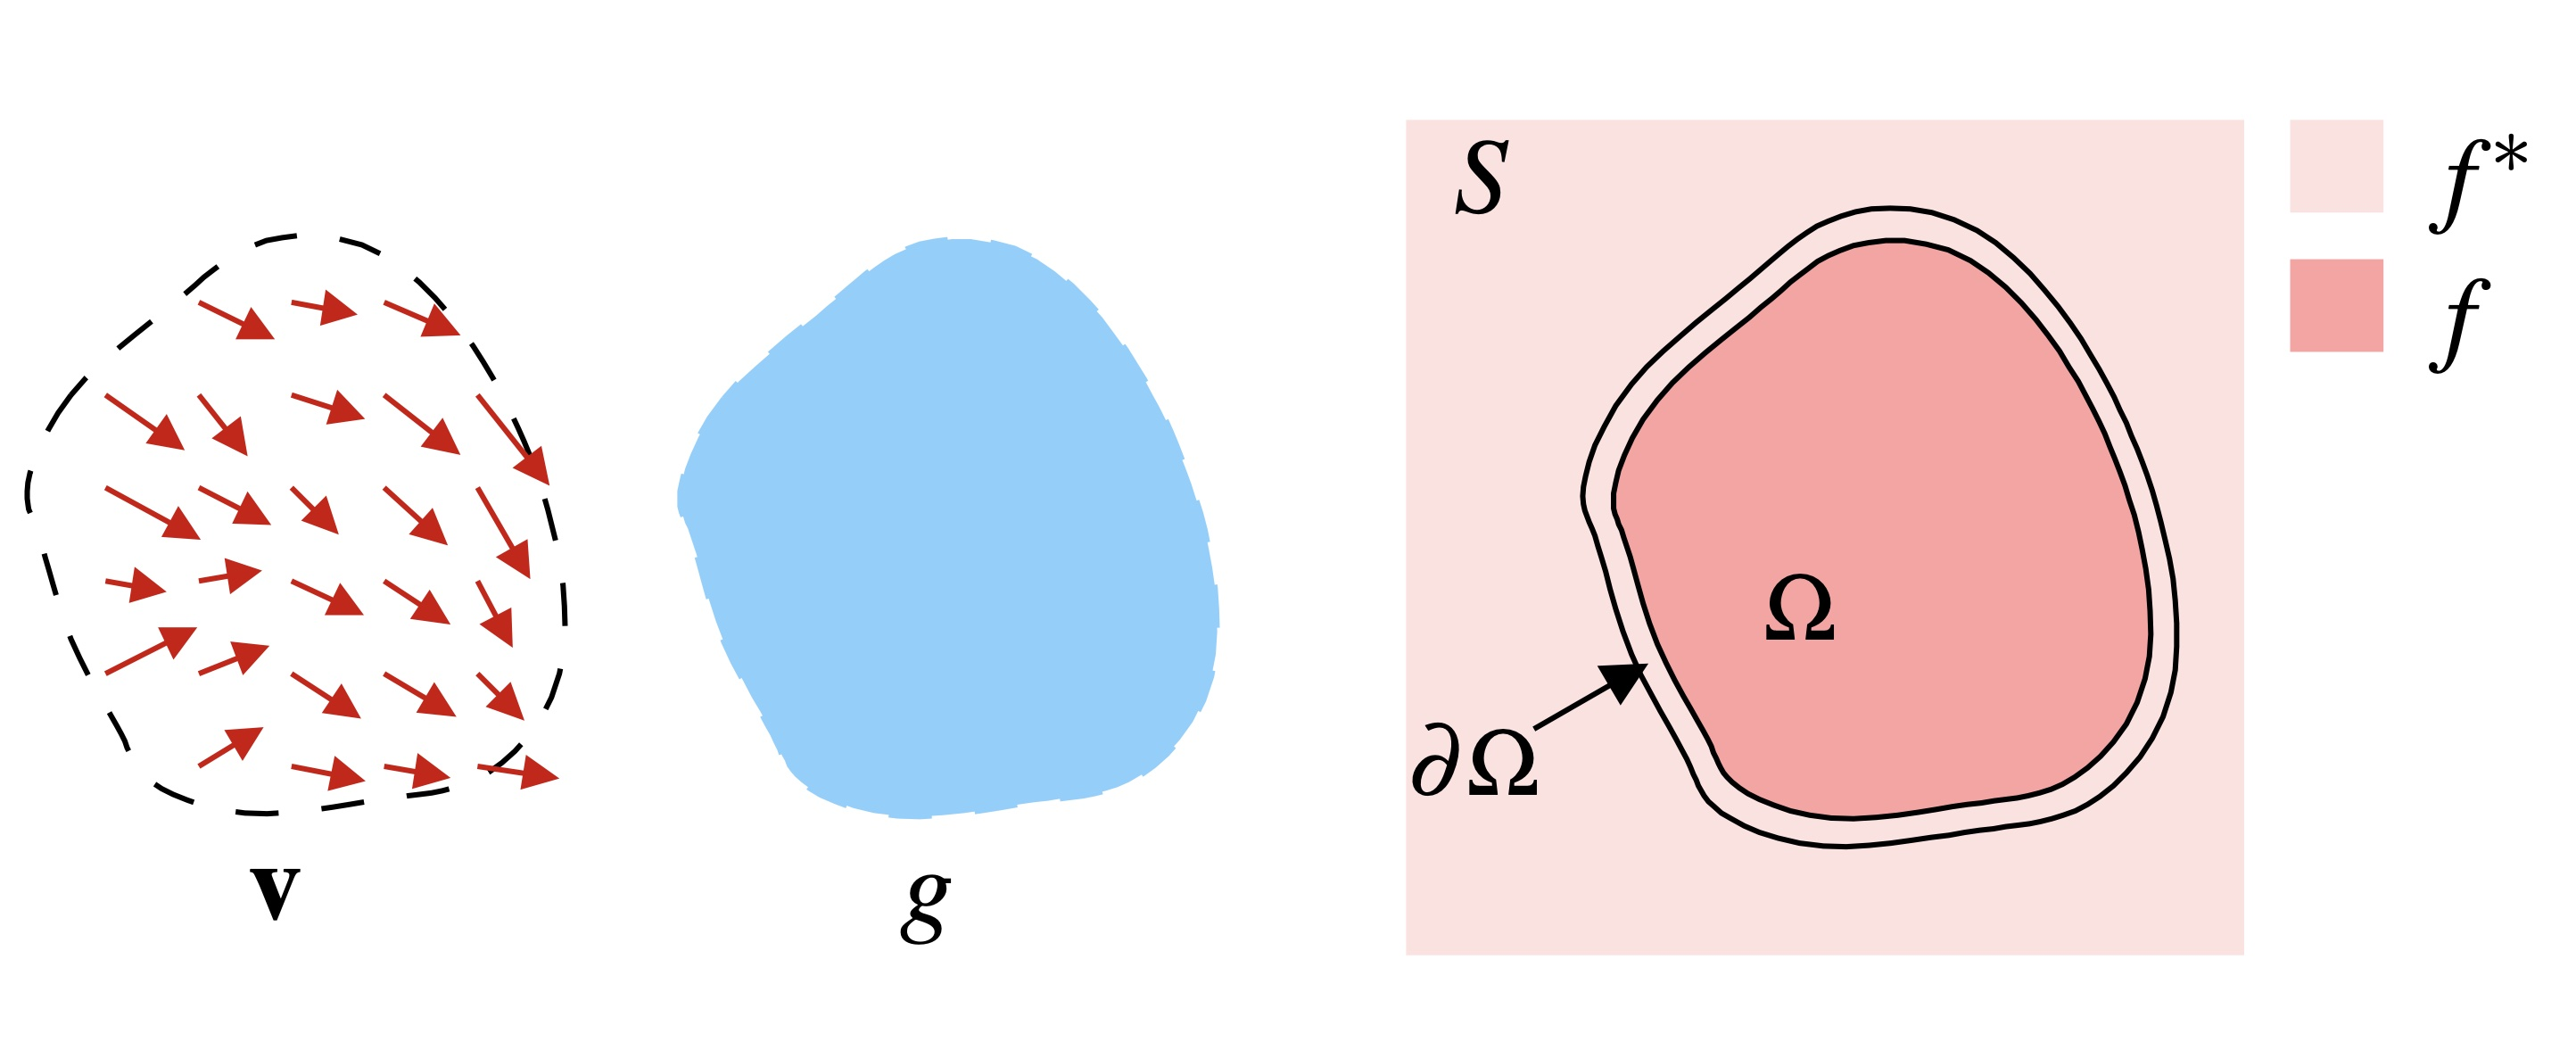
\includegraphics[width = 10cm]{notation.jpg}
\end{center}

let S, a closed subset of R2, be the image definition domain, and let Ω be a closed subset of S with boundary ∂Ω. Let $f^∗$  be a known scalar function defined over S minus the interior of Ω and let f be an unknown scalar function defined over the interior of Ω. Finally, let v be a vector field defined over Ω.
\subsubsection{Membrane interpolation}
 the solution of the minimization problem:
 \begin{equation}
      \min _f \iint_{\Omega}|\nabla f|^2 \text { with }\left.f\right|_{\partial \Omega}=f^* \mid \partial \Omega,
 \end{equation}
 where $\nabla .=\left[\frac{\partial .}{\partial x}, \frac{\partial}{\partial y}\right]$ is the gradient operator. The minimizer must satisfy the associated Euler-Lagrange equation
 \begin{equation}
     \Delta f=0 \text { over } \Omega \text { with }\left.f\right|_{\partial \Omega}=\left.f^*\right|_{\partial \Omega},
 \end{equation}
 where $\Delta .=\frac{\partial^2}{\partial x^2}+\frac{\partial^2}{\partial y^2}$is the Laplacian operator.
 \subsubsection{Minimization with a guidance field}
 an extended version of the above minimization:
 \begin{equation}
     \min _f \iint_{\Omega}|\nabla f-\mathbf{v}|^2 \text { with }\left.f\right|_{\partial \Omega}=\left.f^*\right|_{\partial \Omega},
 \end{equation}
 whose solution is the unique solution of the following Poisson equation with Dirichlet boundary conditions:
 \begin{equation}
     \Delta f=\operatorname{div} \mathbf{v} \text { over } \Omega, \text { with }\left.f\right|_{\partial \Omega}=\left.f^*\right|_{\partial \Omega},
 \end{equation}
 where $\operatorname{div} \mathbf{v}=\frac{\partial u}{\partial x}+\frac{\partial v}{\partial y}$ is the divergence of $\mathbf{v}=(u, v)$.
 This is the fundamental machinery of Poisson editing of color images: three Poisson equations of the form (4) are solved independently in the three color channels of the chosen color space.
\subsection{Discrete Poisson solver}
For discrete images the problem can be discretized naturally using the underlying discrete pixel grid. For each pixel p in S, let $N_p$ be the set of its 4-connected neighbors which are in S, and let ⟨p,q⟩ denote a pixel pair such that q ∈$N_p$. The boundary of Ω is now $\partial \Omega=\{p \in S \backslash \Omega:N_p\cap\Omega\neq0\}$.

The finite difference discretization of (3) yields the following discrete, quadratic optimization problem:
\begin{equation}
    \min _{\left.f\right|_{\Omega}} \sum_{\langle p, q\rangle \cap \Omega \neq \emptyset}\left(f_p-f_q-v_{p q}\right)^2, \text { with } f_p=f_p^* \text {, for all } p \in \partial \Omega.
\end{equation}
Its solution satisfies the following simultaneous linear equations:
\begin{equation}
    \text { for all } p \in \Omega, \quad\left|N_p\right| f_p-\sum_{q \in N_p \cap \Omega} f_q=\sum_{q \in N_p \cap \partial \Omega} f_q^*+\sum_{q \in N_p} v_{p q} .
\end{equation}
For pixels p interior to Ω, that is, Np ⊂ Ω, there are no boundary terms in the right hand side of (6), which reads:
\begin{equation}
    \left|N_p\right| f_p-\sum_{q \in N_p} f_q=\sum_{q \in N_p} v_{p q}
\end{equation}
\subsection{Seamless clone}
\subsubsection{Importing gradients}
The basic choice for the guidance field v is a gradient field taken directly from a source image. 
\begin{equation}
    \Delta f=\Delta g \text { over } \Omega, \text { with }\left.f\right|_{\partial \Omega}=\left.f^*\right|_{\partial \Omega}
\end{equation}
As for the numerical implementation, the continuous specification (8) translates into
\begin{equation}
    for\,all <p,q>, v_{pq}=g_p-g_q
\end{equation}
which is to be plugged into (6).
\subsubsection{Mixing gradients}
 No trace of the destination image $f^∗$ is kept inside Ω with directly importing gradients, but there are situations where it is desirable to combine properties of $f^∗$ with those of g, for example to add objects with holes, or partially transparent ones, on top of a textured or cluttered background.
 
 As a result, at each point of Ω, we retain the stronger of the variations in $f^∗$ or in g, using the following guidance field:
 \begin{equation}
     \text { for all } \mathbf{x} \in \Omega, \mathbf{v}(\mathbf{x})= \begin{cases}\nabla f^*(\mathbf{x}) & \text { if }\left|\nabla f^*(\mathbf{x})\right|>|\nabla g(\mathbf{x})| \\ \nabla g(\mathbf{x}) & \text { otherwise. }\end{cases}.
 \end{equation}
 The discrete counterpart of this guidance field is:
 \begin{equation}
     v_{p q}= \begin{cases}f_p^*-f_q^* & \text { if }\left|f_p^*-f_q^*\right|>\left|g_p-g_q\right| \\ g_p-g_q & \text { otherwise }\end{cases}.
 \end{equation}
\newpage
 \section{Experiment results}
 \subsection{Test-case 1: Cloning Kendall's face onto Kim's }
 \begin{figure}[H]
     \centering
     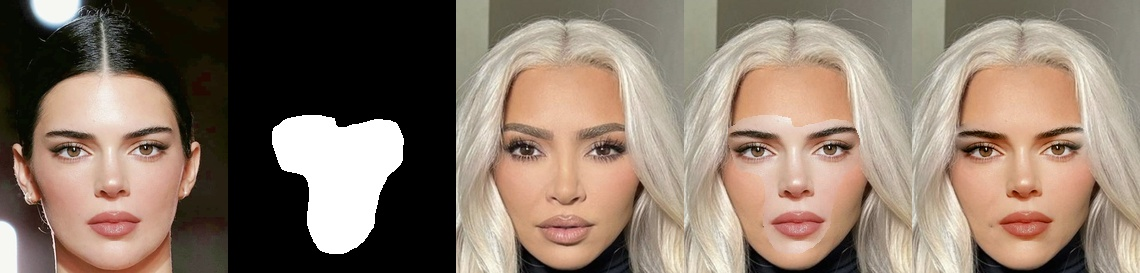
\includegraphics[width=0.9\textwidth]{progress_import_Kardashian.jpg}
     \caption{This is a picture of the progress of cloning Kendall's face onto Kim's using Poisson Image Editing by directly importing gradients.}
     \label{fig:my_label}
 \end{figure}
 \subsection{Test-case 2: Cloning a strawberry onto a chocolate milk shake }
 \begin{figure}[H]
     \centering
     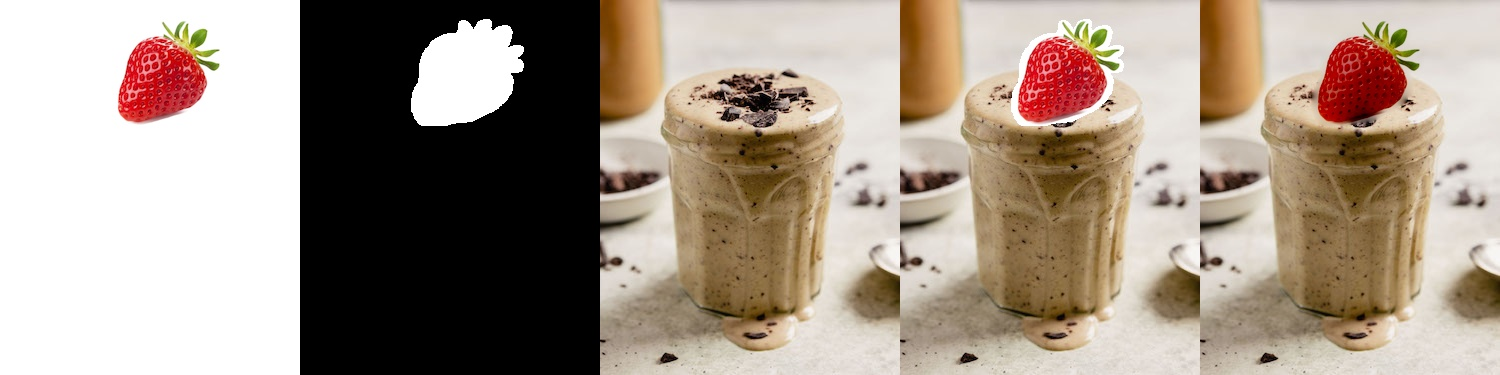
\includegraphics[width=0.9\textwidth]{progress_import_strawberry Milk Shake.jpg}
     \caption{This is a picture of the progress of cloning a strawberry onto a chocolate milk shake using Poisson Image Editing by directly importing gradients.}
     \label{fig:my_label}
 \end{figure}
 \subsection{Test-case 3: Cloning Ginevra de' Benci's face onto Monna Lisa’s}
 \begin{figure}[H]
     \centering
     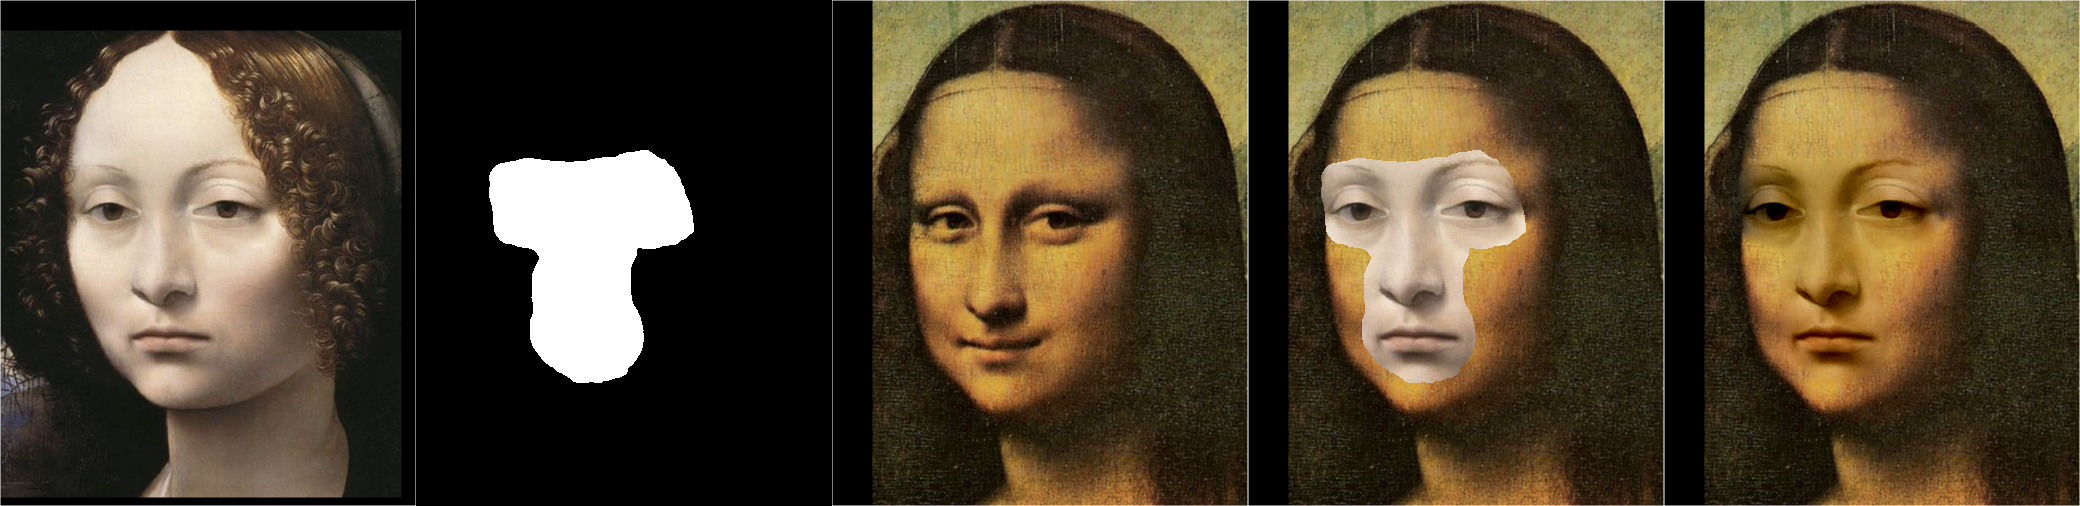
\includegraphics[width=0.9\textwidth]{progress_import_monna.png}
     \caption{This is a picture of the progress of cloning Ginevra de' Benci's face onto Monna Lisa's using Poisson Image Editing by directly importing gradients.}
     \label{fig:my_label}
 \end{figure}
 \subsection{Test-case 4: Inserting object with holes}
 \begin{figure}[H]
     \centering
     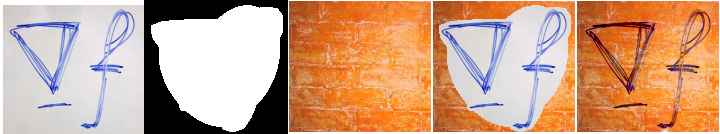
\includegraphics[width=0.9\textwidth]{merged_result_mix.png}
     \caption{This is a picture of the progress of inserting objects with hole using Poisson Image Editing by mixing gradients.}
     \label{fig:my_label}
 \end{figure}
  \begin{figure}[H]
     \centering
     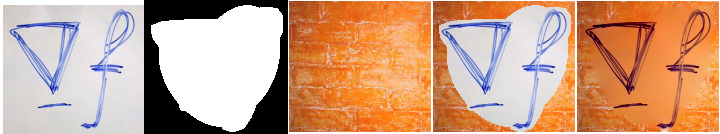
\includegraphics[width=0.9\textwidth]{merged_result_import.png}
     \caption{This is a picture of the progress of inserting objects with hole using Poisson Image Editing by directly importing gradients.}
     \label{fig:my_label}
 \end{figure}
 \subsection{Test-case 5:Replacing a doughnut with hamburger}
 \begin{figure}[H]
     \centering
     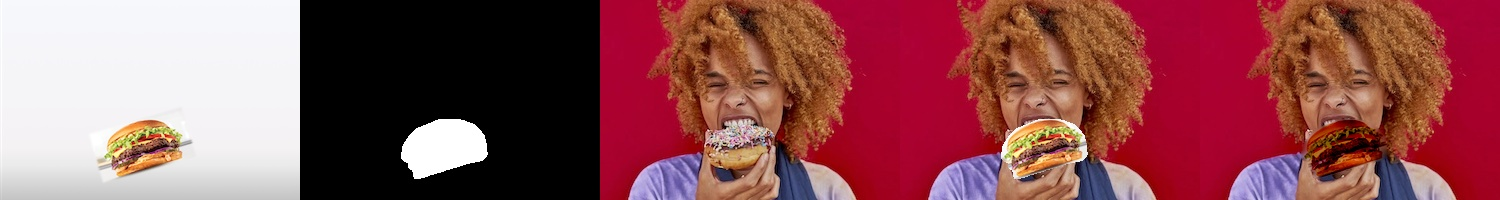
\includegraphics[width=1.1\textwidth]{progress_import.jpg}
     \caption{This is a picture of the progress of replacing a doughnut with hamburger using Poisson Image Editing by mixing gradients.}
     \label{fig:my_label}
 \end{figure}
 \newpage
 \section{Algorithm implementation}
 \subsection{Run}
 Before running the main.py file, you need to configure the launch.json file in .vscode folder in order to send in the arguments.There are 5 test cases in the test folder
 \begin{lstlisting}[language=python]
 "args": [
                "/Users/mac/Repo/PosisonImageEditing/test/test5/source.png",
                "/Users/mac/Repo/PosisonImageEditing/test/test5/mask.png",
                "/Users/mac/Repo/PosisonImageEditing/test/test5/target.jpg",
                "import"
            ]
 \end{lstlisting}
\subsection{Preprocessing}
 \subsubsection{Extracting outline of mask image}
 \begin{lstlisting}[language=python]
def get_outline(NormalizedMask_npArr):
  Mask_01Arr = np.array(NormalizedMask_npArr, dtype=np.uint8)
  ErodedMask_01Arr = cv.erode(Mask_01Arr, np.ones((3, 3), np.uint8))
  Outline = Mask_01Arr * (1 - ErodedMask_01Arr) 

  return Outline
 \end{lstlisting}
 This is done by erode the mask image and multiply the mask's numpy array with the "reversed" eroded mask numpy array.
 \subsubsection{Indicing}
 \begin{lstlisting}[language=python]
 def indicies(NormalizedMask_npArr):
  # height and width of mask image
  Height, Width = NormalizedMask_npArr.shape

  # index of omega area
  Omega = np.nonzero(NormalizedMask_npArr)
  RowIDArr = Omega[0]
  ColIDArr = Omega[1]
  RowIDvec = np.reshape(RowIDArr, [RowIDArr.shape[0], 1])
  ColIDvec = np.reshape(ColIDArr, [ColIDArr.shape[0], 1])
  OmegaCoordinateArr = np.concatenate([RowIDvec, ColIDvec], 1)

  ## 1. flag of neigbourhoods pixel.
  ## --> write TRUE if neigbourhoods pixel is exist, FALSE otherwise.
  ## 2. dictionary for omega's index
  Neighborhoods_existence = []
  NumberedOmega = np.zeros((Height, Width), dtype=np.int32)
  for i in range(OmegaCoordinateArr.shape[0]):

    # pixel coordination
    RowID, ColID = OmegaCoordinateArr[i]

    # record the existence of neighborhood 
    Neighborhoods_existence.append([check_existence(NormalizedMask_npArr, RowID, ColID+1),
                     check_existence(NormalizedMask_npArr, RowID, ColID-1),
                     check_existence(NormalizedMask_npArr, RowID+1, ColID),
                     check_existence(NormalizedMask_npArr, RowID-1, ColID),])

    ## numebr the Omega are(0,1,2....)
    NumberedOmega[RowID][ColID] = i

  return OmegaCoordinateArr, np.array(Neighborhoods_existence), NumberedOmega
 \end{lstlisting}
 This part mainly do 3 things, the first thing is indexing the $\Omega$ area, the second thing is checking the existence of the respectively right, left, up and bottom neighborhood, and give each pixel in $\Omega$ an ID. 
 \subsection{Computing coefficient matrix A}
 \begin{lstlisting}[language=python]
 def coefficient_matrix(OmegaCoordinateArr, Neighborhood_existence, NumberedOmega, A, OmegaDim):
  for i in range(OmegaDim):

    ## progress bar
    progress_bar(i, OmegaDim-1)

    ## fill 4 or -1(Laplacian kernel)
    A[i, i] = 4
    RowID, ColID = OmegaCoordinateArr[i]

    ## right
    if(Neighborhood_existence[i][0]):
      j = NumberedOmega[RowID][ColID+1]
      A[i, j] = -1

    ## left
    if(Neighborhood_existence[i][1]):
      j = NumberedOmega[RowID][ColID-1]
      A[i, j] = -1

    ## bottom
    if(Neighborhood_existence[i][2]):
      j = NumberedOmega[RowID+1][ColID]
      A[i, j] = -1

    ## up
    if(Neighborhood_existence[i][3]):
      j = NumberedOmega[RowID-1][ColID]
      A[i, j] = -1

  return A
 \end{lstlisting}
 For pixels inside $\Omega$ area, using Laplacian kernel to serve as coefficient.
 \begin{figure}[H]
     \centering
     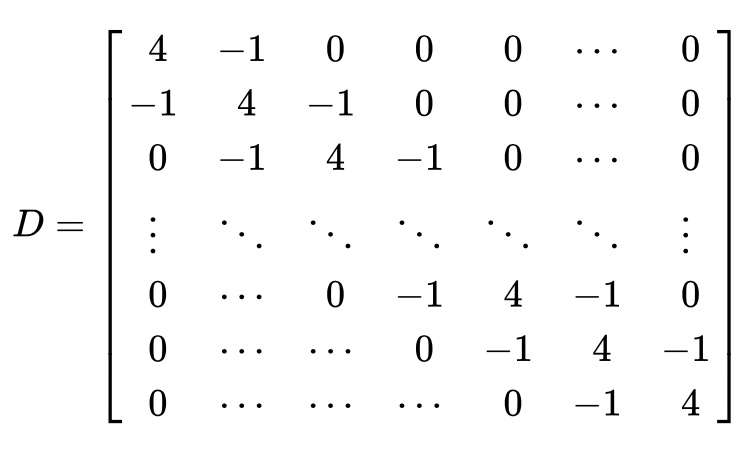
\includegraphics[width=0.6\textwidth]{LaplacianOperator.jpg}
     \caption{Laplacian operator}
     \label{fig:my_label}
 \end{figure}
 \begin{figure}[H]
     \centering
     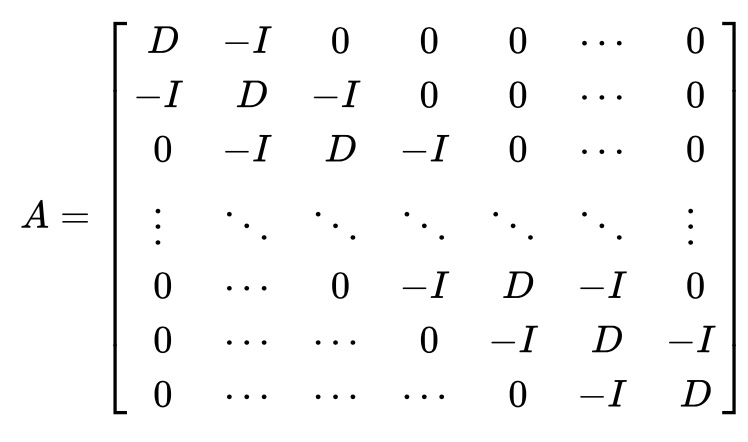
\includegraphics[width=0.6\textwidth]{Amatrix.jpg}
     \caption{Coefficient matrix A, where I is identity matrix, and D is given by figure 7}
     \label{fig:my_label}
 \end{figure}
 \subsection{Computing vector u in Ax = u}
 \subsubsection{Directly importing gradients}
 \begin{lstlisting}[language=python]
def importing_gradients(NormalizedSrcImg_npArr, NormalizedTargetImg_npArr, OmegaCoordinateArr, Outline, Neighborhood_existence, OmegaDim):
  ### output array
  u_R = np.zeros(OmegaDim)
  u_G = np.zeros(OmegaDim)
  u_B = np.zeros(OmegaDim)

  ### take laplacian
  for i in range(OmegaDim):

    ## progress
    progress_bar(i, OmegaCoordinateArr.shape[0]-1)

    ## apply each color channel
    u_R[i] = laplacian_at_coordinate_import(NormalizedSrcImg_npArr[:, :, 2], OmegaCoordinateArr[i], Neighborhood_existence[i]) \
                  + constrain(NormalizedTargetImg_npArr[:, :, 2], OmegaCoordinateArr[i], Outline, Neighborhood_existence[i])
    u_G[i] = laplacian_at_coordinate_import(NormalizedSrcImg_npArr[:, :, 1], OmegaCoordinateArr[i], Neighborhood_existence[i]) \
                  + constrain(NormalizedTargetImg_npArr[:, :, 1], OmegaCoordinateArr[i], Outline, Neighborhood_existence[i])
    u_B[i] = laplacian_at_coordinate_import(NormalizedSrcImg_npArr[:, :, 0], OmegaCoordinateArr[i], Neighborhood_existence[i]) \
                  + constrain(NormalizedTargetImg_npArr[:, :, 0], OmegaCoordinateArr[i], Outline, Neighborhood_existence[i])

  return  u_R , u_G, u_B
 \end{lstlisting}
 This is done by directly importing Laplacian of the source image.
 \subsubsection{Mixing gradients}
 \begin{lstlisting}[language=python]
 def mixing_gradients(NormalizedSrcImg_npArr, NormalizedTargetImg_npArr, OmegaCoordinateArr, Outline, Neighborhood_existence, OmegaDim):
  ## array for 3 color channel
  u_R = np.zeros(OmegaDim)
  u_G = np.zeros(OmegaDim)
  u_B = np.zeros(OmegaDim)

  ## calculate laplacian
  for i in range(OmegaDim):

    ## progress
    progress_bar(i, OmegaDim-1)

    ## apply each color channel
    u_R[i] = laplacian_at_coordinate_mix(NormalizedSrcImg_npArr[:, :, 2], NormalizedTargetImg_npArr[:, :, 2], OmegaCoordinateArr[i], Neighborhood_existence[i]) \
                + constrain(NormalizedTargetImg_npArr[:, :, 2], OmegaCoordinateArr[i], Outline, Neighborhood_existence[i])
    u_G[i] = laplacian_at_coordinate_mix(NormalizedSrcImg_npArr[:, :, 1], NormalizedTargetImg_npArr[:, :, 1], OmegaCoordinateArr[i], Neighborhood_existence[i]) \
                + constrain(NormalizedTargetImg_npArr[:, :, 1], OmegaCoordinateArr[i], Outline, Neighborhood_existence[i])                  
    u_B[i] = laplacian_at_coordinate_mix(NormalizedSrcImg_npArr[:, :, 0], NormalizedTargetImg_npArr[:, :, 0], OmegaCoordinateArr[i], Neighborhood_existence[i]) \
                + constrain(NormalizedTargetImg_npArr[:, :, 0], OmegaCoordinateArr[i], Outline, Neighborhood_existence[i])
             
  return u_R, u_G, u_B
 \end{lstlisting}
 This is done by importing the greater value of the gradient of the source image and the target image, and use that to compute Laplacian at the right-hand-side. 
 \subsubsection{Dirichlet boundary condition}
 \begin{lstlisting}[language=python]
def constrain(AChannelOf_NormalizedTargetImg, OmegaCoordinate, Outline, Neighborhood_existence):
  '''
  Function to set grad(source) = target at boundary
  return Dirichlet boundary condition for Coordinate
  '''
  ## current coordinate
  RowID, ColID = OmegaCoordinate

  ## In order to use "Dirichlet boundary condition",
  ## if on boundry, add in target intensity --> set constraint grad(source) = target at boundary
  if(Outline[RowID][ColID]==1):#if current pixel is on boundary
    val = (float(Neighborhood_existence[0]==False) * AChannelOf_NormalizedTargetImg[RowID, ColID+1]#right
           + float(Neighborhood_existence[1]==False) * AChannelOf_NormalizedTargetImg[RowID, ColID-1]#left
           + float(Neighborhood_existence[2]==False) * AChannelOf_NormalizedTargetImg[RowID+1, ColID]#bottom
           + float(Neighborhood_existence[3]==False) * AChannelOf_NormalizedTargetImg[RowID-1, ColID])#up
    return val

  ## If not on boundry, just take laplacian.
  else:#Outline[RowID][ColID]==0
    val = 0.0
    return val
 \end{lstlisting}
However, if the pixel dealing with is on the boundary, it doesn't have all of its 4 neighbor, so we cannot compute its Laplacian, so what we are going to do is use Dirichlet boundary condition to complement the missing neighborhood, which is done add target image's intensity value into the vector u.
\begin{figure}[H]
    \centering
    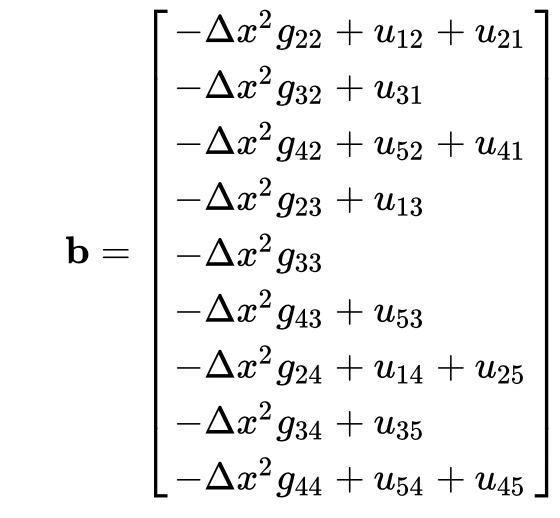
\includegraphics[width=0.4\textwidth]{UwithDirichlet.jpg}
    \caption{Example of vector u with Dirichlet condition, in vector u the $u_{i,j}$ will be the intensity value of target image}
    \label{fig:my_label}
\end{figure}
 \subsection{Solving x in Ax = u}
 \begin{lstlisting}[language=python]
  ### Matrix computing
  print("step3: solve Ax = u")

  x_R, _ = sp.linalg.cg(A, u_R)
  x_G, _= sp.linalg.cg(A, u_G)
  x_B, _ = sp.linalg.cg(A, u_B)

  print("done!\n")
 \end{lstlisting}
 Since matrix computing is not the concentration of this assignment, I just call the package linalg.cg in scipy.sparse to do the work.
 \newpage
 \section{My thinking}
 \subsection{Problems and solutions}
 I think the biggest challenge I faced is the mathematical formula in the Poisson Image Editing paper, I feel like I am an idiot when I first run into it, and it felt terrible. I struggled through it by looking up tutorials about Poisson Image Editing in Zhihu, and it started to make sense, and I read that paper over and over, and constantly learning the mathematical concept in Wikipedia
 \subsection{Future work}
I think the mask's shape has a relatively significant influence on the result of Poisson Image Editing, so I think it will be a good direction to spare effort.
 
%%%%%%%%%%%%%%%%%%%%%%%%%%%%%%%%%%%%%%%%%%%%%%%%%%%%%%%%%%%%
%Complete the assignment now
\end{document}
